\documentclass{beamer}
\usepackage[utf8]{inputenc}
\usepackage[czech]{babel}
\usepackage{hyperref}
\usepackage{listings}
\usepackage{setspace}

\usetheme{Warsaw}
\urlstyle{same}

\title{Datová structura "Pole"}
\subtitle{v jazyce C/C++}
\author{Ivan Tsiareshkin}
\institute{Fakulta Informačních technologií\\Vysoké učení technické v Brně}
\date{\today}

\begin{document}

\frame{\titlepage}

\begin{frame}{Definice}
\begin{itemize}
    \item \onslide<1->{Pole je kolekce prvků stejného typu, na která lze jednotlivě odkazovat pomocí indexu k jedinečnému identifikátoru.}
    \item \onslide<1->{Pět hodnot typu int lze deklarovat jako pole, aniž byste museli deklarovat pět různých proměnných.}
\end{itemize}
\end{frame}

\begin{frame}{Příklad}
    \begin{flushleft}
    Například pětičlenné pole foo může být logicky reprezentováno jako:
    \end{flushleft}
    \begin{center}
    \scalebox{0.6}{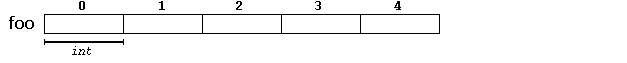
\includegraphics{1.jpg}}\\[1em]
    \end{center}
    \begin{flushleft}
    kde každá prázdná buňka představuje prvek pole.
    V tomto případě se jedná o hodnoty typu int.
    Tyto prvky jsou očíslovány od 0 do 4, přičemž 0 je první, zatímco 4 jsou poslední.
    V jazyce C/C++ je index prvního prvku pole vždy nula.
    \end{flushleft}
\end{frame}


\begin{frame}{Pseudokód deklarace a inicializace}
    \begin{flushleft}
        type name [elements]; - deklarace
        \\
        type name [elements] = \{\,\}; - inicializace
        \\
        Tím se vytvoří pole hodnot, z nichž každá je inicializována na nulu.
    \end{flushleft}
\end{frame}

\begin{frame}{Deklarace a inicializace}
    Ale prvky v poli lze inicializovat na konkrétní hodnoty, uzavřením těchto počátečních hodnot do složených závorek \{\}. Například:
    \\
    int foo [5] = \{\ 16, 2, 77, 40, 12071 \};
    \\
    \begin{center}
    \scalebox{0.6}{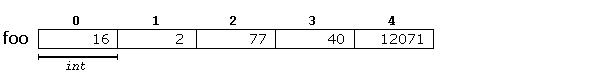
\includegraphics{2.jpg}}\\[1em]
    \end{center}
\end{frame}

\begin{frame}{Deklarace a inicializace}
    Počet hodnot mezi složenými závorkami nesmí být větší než počet prvků v poli. Například ve výše uvedeném příkladu bylo foo deklarováno s 5 prvky a složené závorky obsahovaly přesně 5 hodnot, jednu pro každý prvek.
\end{frame}

\begin{frame}{Přistup k poli}
    \begin{flushleft}
    K hodnotám kteréhokoli z prvků v poli lze přistupovat stejně jako k hodnotě běžné proměnné stejného typu. Syntaxe je:
        \begin{center}
            jméno [index]
        \end{center}
    Po předchozím příkladu, ve kterém foo mělo 5 prvků a každý z těchto prvků byl typu int, je název, kterým lze odkazovat na každý prvek, následující:
        \begin{center}
        \scalebox{0.5}{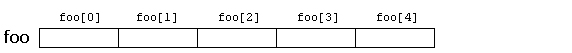
\includegraphics{3.jpg}}\\[1em]
        \end{center}
    Například následující příkaz uloží hodnotu 75 ve třetím prvku foo:
        \begin{center}
            foo [2] = 75;
        \end{center}

    A například následující kopíruje hodnotu čtvrtého prvku foo do proměnné s názvem x:
        \begin{center}
            x = foo [3];
        \end{center}
    \end{flushleft}
\end{frame}

\begin{frame}{Příklad práce s polem}
    \lstinputlisting[language=C]{code.c}
\end{frame}



\begin{frame}{Vícerozměrná pole}
    \begin{flushleft}
        Vícerozměrná pole lze popsat jako „pole polí“.
        Například dvourozměrné pole si lze představit jako dvourozměrnou tabulku vytvořenou z prvků obsahujících prvky stejného typu.
        \begin{center}
            \scalebox{0.5}{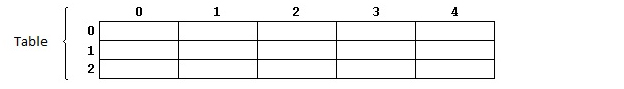
\includegraphics{4.jpg}}\\[1em]
        \end{center}\textbf{}
    \end{flushleft}
\end{frame}

\begin{frame}{Vícerozměrná pole}
   \begin{flushleft}
        Tabulka je dvourozměrné pole 3 až 5 int prvků. Syntaxe C/C++:
         \begin{center}
            int Tabulka [3][5];
         \end{center}
        Způsob odkazu na druhý prvek svisle a čtvrtý vodorovně ve výrazu by byl následující:
        \begin{center}
            Tabulka [1][3]
        \end{center}
    \end{flushleft}
\end{frame}

\begin{frame}{Vícerozměrná pole}
    \begin{flushleft}
        Vícerozměrná pole nejsou omezena na dva indexy.
        Mohou obsahovat tolik indexů, kolik chcete, ale množství paměti potřebné pro pole se exponenciálně zvyšuje s každou dimenzí. Například:
        \begin{center}
           char century [100][365][24][60][60];
        \end{center}
        Deklaruje pole s char prvkem na každou sekundu během století. To je více než 3 miliardy znaků. Tento operátor tedy spotřebovává více než 3 gigabajty paměti. A takové prohlášení je nepravděpodobné a zdůrazňuje neefektivní využití paměťového prostoru.
    \end{flushleft}
\end{frame}

\begin{frame}{Použité zdroje}
\begin{itemize}
\setlength{\parskip}{0.10em}
    \item ARRAYS IN C++ \\[0.2em]
    \small{\url{https://www.cpp.edu/~elab/ECE114/Array.html}}
\end{itemize}
\end{frame}

\end{document}\textbf{}
